\section{Step Length}
\fxnote{skal måske være i subsection sammen med finding steps}
When the steps have been found, the next task is to determine the length of the step.
The length is determined by the area under the velocity graph for one step, as seen in \figref{figure:area}.
The area is found by taking the integral of the velocity graph,
$$s = \int (v)\mathrm{d}t$$
where $v$ is the velocity and $s$ is the area under the graph.
 %nyt billede her!
\begin{figure}[h]
	\centering	
	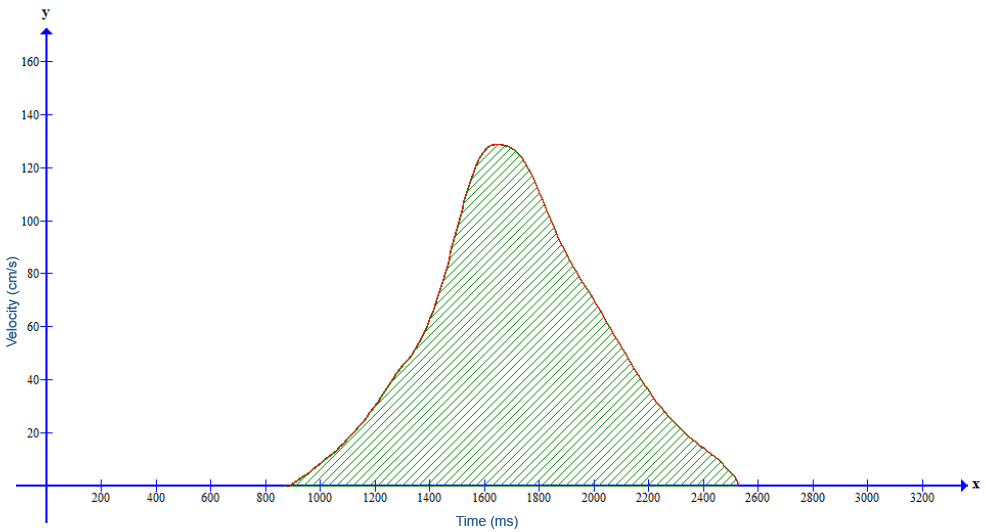
\includegraphics[scale=0.4]{media/area3}
	\caption{The area between the velocity graph and local-extrema-intersecting graph}
	\label{figure:area}
\end{figure}

This area can then be used to determine the steps actual length and used to move the paddle in the game.
The area per step graph, \figref{}, is made by looking at video footage of people using the accelerometer and comparing their actual step length with the area found.